\chapter{Algebra Review}
This is a draft chapter of the course manual and is not comprehensive. Many of the skills used in this chapter are foundational mathematical tools that you will need to keep using repeatedly both in this course and beyond. Refer to the course website $<$\texttt{blackboard.aut.ac.nz}$>$ for additional review material covering the basics of algebra.

 \section{Linear Functions}
 Slope of a line is often represented by the letter $m$ and can be calculated by taking any two points on the line $(x_1,y_1)$, and $(x_2,y_2)$ and using the formula: $m =\frac{y_{2} -y_{1}}{x_{2} -x_{1}}$.
 
 The standard form for an equation of a line is: $y =m x +c$ where $m$ is the slope described above, and $c$ is the $y-$intercept. Alternatively if you know the slope and any given point $(x_1,y_1)$, the equation of a line is $y -y_{1} =m (x -x_{1})$.

\section{Distance between two points}
Using the Pythagorean theorem, the distance between two points $\left (x_{1} .y_{1}\right )$ and $\left (x_{2} .y_{2}\right )$ is $$\text{dist}=\sqrt{\left (x_{1} -x_{2}\right )^{2} +\left (y_{1} -y_{2}\right )^{2}}$$ 

 \section{Quadratic Functions}
 The standard for of a quadratic equation is written $a x^{2} +b x +c =0$. If we solve this equation for $x$ we get the quadratic formula:
 $$x =\frac{ -b \pm \sqrt{b^{2} -4 a c}}{2 a}$$ 
 where $a,b,$ and $c$ are coefficients ($a\ne0$). Note here there are two possible solutions because of the plus-minus sign ($\pm$).
 
 \section{Factorising}
 We usually use the word factorising in New Zealand however most textbooks use the term factoring. We will use both terms interchangeably in this course. Factor(is)ing is a fundamental skill that students must master.  
 
 Multiplying algebraic expressions is usually called \emph{expanding}
 and the reverse process is called \emph{factorising}. This process of factorising is usually
 taught by going through many examples until patterns can be seen. You should carefully look at the examples posted on blackboard if you need to see how factorising is done. 
 
 \subsubsection{Example}
 Factorise: $x^{2} -5 x -6$ 
 
 For these examples you are required to find a pair of numbers that add together to give $ -5$ and multiply together to give $ -6$. In this case the numbers are $ -6$ and $ +1$. So the answer is
 \begin{equation*}x^{2} -5 x -6 =\left (x -6\right ) \left (x +1\right )
 \end{equation*}
 
 This can easily be verified by expanding the brackets. 
 \section{Exponential and Logarithmic Functions}
 Laws of logarithms. This will be covered in detail in Chapter 4.\\
 $\log _{a} X Y =\log _{a} X +\log _{a} Y$ 
 
 $\log _{a} \genfrac{(}{)}{}{}{X}{Y} =\log _{a} X -\log _{a} Y$ 
 
 $\log _{a} X^{n} =n \log _{a} X$ 
 
 
\section{Foundation Algebra Exercises} 
 
\begin{enumerate}
	\item Remove the brackets 
	\begin{enumerate}
		\item $ -\left (x +y\right )$ 
		\item $ -3 (5 x -2 y)$ \end{enumerate}
	
	\item Evaluate $\left (\frac{1}{3} \div \frac{1}{6}\right ) +\frac{1}{2}$ 
	
	\item Calculate the value of 
	\begin{enumerate}
		\item $\left (15.3\right )^{0}$ 
		\item $10^{ -2}$ \end{enumerate}
	\item Simplify 
	\begin{enumerate}
		\item $\left (3 a^{2} b\right )^{2}$ 
		
		\item $\genfrac{(}{)}{}{}{x}{3}^{3} x^{3}$ \end{enumerate}
	
	
	\item Evaluate $\sqrt[{4}]{2.7}$ accurate to 2 decimal places. 
	
	\item Remove the brackets and simplify 
	
	
	\begin{enumerate}
		\item $\left (x^{2} +5 x -1\right ) -\left (2 x -3\right )$ 
		
		\item $\left (2 x -1\right ) \left (2 x +1\right )$ \end{enumerate}
	
	
	\item Factorise the expressions 
	\begin{enumerate}
		\item $x^{2} +11 x +28$ 	
		\item $2 x^{2} -5 x -12$ 
		\end{enumerate}
	\item Simplify $\frac{x^{2} +5 x +6}{x^{2} +2 x -3}$ by factorising and then cancelling 
	
	\item Solve the equations 
	
	
	\begin{enumerate}
		\item $7 x -16 =\frac{2}{3} x +4$ 
		
		\item $\left (x -2\right )^{2} =15$ \end{enumerate}

	\item Solve the equations 
	
	
	\begin{enumerate}
		\item $x^{2} -2 x -8 =0$ by factorising. 
		
		\item $2 x^{2} +5 x -4 =0$ by using the quadratic formula. \end{enumerate}
	
	
	\item
	Make $t$ the subject of the equation 
	
	
	\begin{enumerate}
		\item $v =u +a t$ 
		
		\item $l =l_{0} \left (1 +\alpha  t\right )$ \end{enumerate}
	
	
	\item 
	The volume of a pipe with length $l$, inner radius $r$ and outer radius $R$ is $V =\pi  \left (R^{2} -r^{2}\right ) l\text{.}$ Find the volume when $R =3.1 \mbox{m}$, $r =2.2 \mbox{m}$ and $l =5.3 \mbox{m}\text{.}$ 
	
	\item  Draw the graph of $y =x^{2} -3$ 
	
	\item  Find the distance between the points $\left (2 , -3\right )$ and $\left (5 , -1\right )\text{.}$ 
	
	\item  Find the $x$ and $y$ intercepts for the graph of $y =x^{2} -3.\vspace{+5.000000cm}$ 
	
	\item    
	\setlength\fboxrule{0in}\setlength\fboxsep{0.2in}\fcolorbox[HTML]{000000}{FFFFFF}{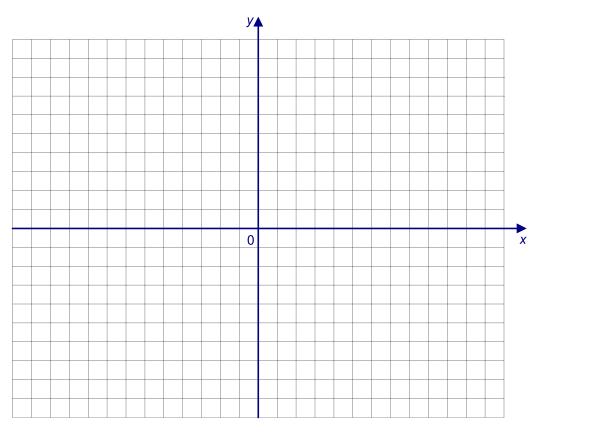
\includegraphics[ width=4.8663in, height=3.4956in,]{L4SZ2705}
	}
	\begin{enumerate}
		\item Show the points $A \left (3 ,5\right )$ and $B \left ( -2 , -5\right )$ on the graph. 
		
		\item Calculate the slope of the line through $A$ and $B$. i.e. the slope of $\bar{AB}\text{.}$ 
		
		\item What is the equation of the line $A B$? 
		
		\item What is the equation of the line parallel to the line $A B$ through the point $\left ( -2 ,3\right )\text{?}$ 
		
		\item Starting from the point $B$ on the graph frame draw a line with a slope of $\frac{4}{5}\text{.}$ 
	\end{enumerate}

  	
	\item 
	If $f (x) =x^{2}$ and $g (x) =x^{3}$ evaluate 
	
	
	\begin{enumerate}
		\item $f (2)$ 
		
		\item $f ( -2)$ 
		
		\item $g (3)$ 
		
		\item $g ( -3)\vspace{+5.000000cm}$ \end{enumerate}
	
	
	\item 
	Complete the table of values for the function $g (x) =x^{3} -x$ and sketch the graph\vspace{0.5cm} \\\relax
	\begin{tabular}[c]{cc}\hline
		$x$  & $g (x) =x^{3} -x$  \\
		\hline
		$ -1.5\rule[-8pt]{0pt}{24pt}$  & \ \ \ \ \ \ \ \ \ \ \ \ \ \ \ \ \ \ \  \\
		\hline
		$ -1\rule[-8pt]{0pt}{24pt}$  &  \\
		\hline
		$ -0.5\rule[-8pt]{0pt}{24pt}$  &  \\
		\hline
		$0\rule[-8pt]{0pt}{24pt}$  &  \\
		\hline
		$0.5\rule[-8pt]{0pt}{24pt}$  &  \\
		\hline
		$1\rule[-8pt]{0pt}{24pt}$  &  \\
		\hline
		$1.5\rule[-8pt]{0pt}{24pt}$  &  \\
		\hline
	\end{tabular} \\\relax
	\setlength\fboxrule{0in}\setlength\fboxsep{0.2in}\fcolorbox[HTML]{000000}{FFFFFF}{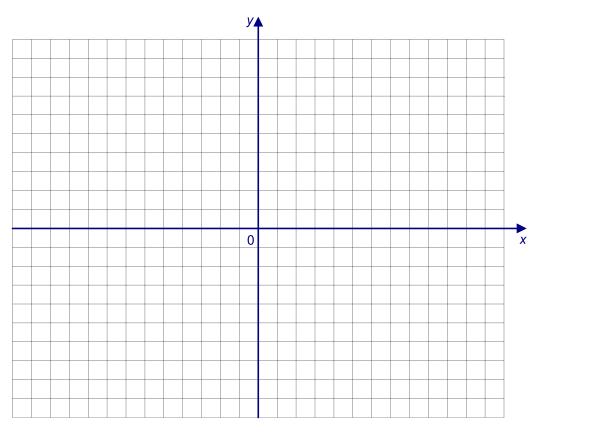
\includegraphics[ width=4.8663in, height=3.4956in,]{L4SZ2706}
	}
	 
	
	\item  Given $f (x) =\left (x +3)(x -1\right )\left (x +1\right )^{2}$ 
	

	\begin{enumerate}
		\item What is the degree of the polynomial? 
		
		\item Where does
		the graph cut the $x$-axis? (I.e. what are the zeros?) 
		
		\item Where does the graph cut the $y$-axis? 
		
		\item Sketch the graph \\\relax
		\setlength\fboxrule{0in}\setlength\fboxsep{0.2in}\fcolorbox[HTML]{000000}{FFFFFF}{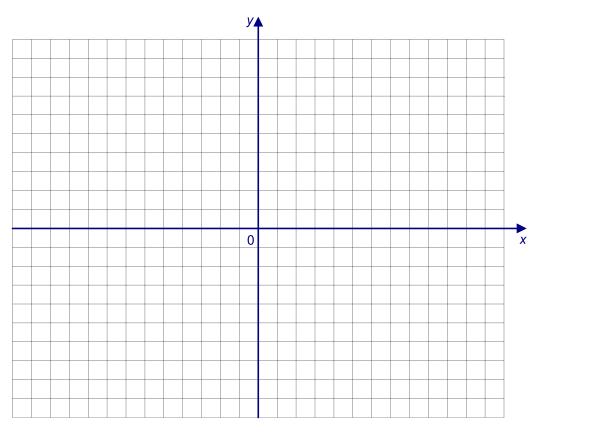
\includegraphics[ width=4.561in, height=3.2759in,]{L4SZ2707}
		}
	\end{enumerate}

	\item Fill in the
	table and draw the graph of $y =\genfrac{(}{)}{}{}{1}{2}^{x}\vspace{+0.500000cm}$ \\\relax
	\begin{tabular}[c]{|c|c|c|c|c|c|c|c|}\hline
		$x$  & -3  & -2  & -1
		& 0  & 1  & 2  & 3
		\\
		\hline
		$y =\genfrac{(}{)}{}{}{1}{2}^{x}$  & \ \ \ \ \ \rule[-8pt]{0pt}{24pt}
		& \ \ \ \ \ \rule[-8pt]{0pt}{24pt}
		& \ \ \ \ \ \rule[-8pt]{0pt}{24pt}
		& \ \ \ \ \ \rule[-8pt]{0pt}{24pt}
		& \ \ \ \ \ \rule[-8pt]{0pt}{24pt}
		& \ \ \ \ \ \rule[-8pt]{0pt}{24pt}
		& \ \ \ \ \ \rule[-8pt]{0pt}{24pt}
		\\
		\hline
	\end{tabular} \\\relax
	\setlength\fboxrule{0in}\setlength\fboxsep{0.2in}\fcolorbox[HTML]{000000}{FFFFFF}{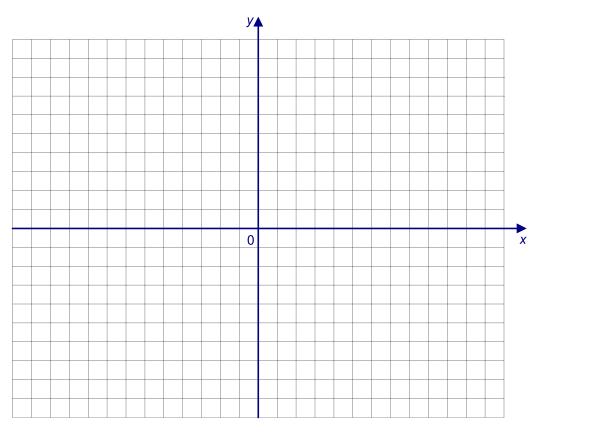
\includegraphics[ width=4.4771in, height=3.2162in,]{L4SZ2708}
	}
	
	
	
	\begin{enumerate}
		\item [(b)] Evaluate 
		
		
		\begin{enumerate}
			\item $3^{3.4}$ 
			
			\item $e^{ -0.6}$ \end{enumerate}
	\end{enumerate}
	
	
	\item 
	Write the equivalent logarithm statement. One is done for you. 
	
	
	\begin{enumerate}
		\item
		\begin{enumerate}
			\item $64 =2^{6} \Leftrightarrow \log _{2} 64 =6$ 
			
			\item $0.01 =10^{ -2} \Leftrightarrow $ \end{enumerate}
		
		
		\item [(b)]
		Write the equivalent statement using an exponent. 
		
		
		\begin{enumerate}
			\item $\log _{5} 625 =4 \Leftrightarrow $ 
			
			\item $\log _{a} k =t \Leftrightarrow $ \end{enumerate}
		
		
		\item [(c)]
		Calculate the value for 
		
		
		\begin{enumerate}
			\item $\log _{9} 9$ 
			
			\item $\log _{2} \genfrac{(}{)}{}{}{1}{8}$ 
			
			\item $\log  1000$ 
			
			\item $\ln  2.95$ 
			
			\item $\ln  e^{3.1}$ 
			
			\item $\log _{4} 0.25$ \end{enumerate}
	\end{enumerate}

	\item Write the following as the logarithm of a single number 
	
	
	\begin{enumerate}
		\item $\log _{4} 7 +\log _{4} 5$ 
		
		\item $\log _{5} 18 -\log _{5} 3$ 
		
		\item $2 \log _{3} 4$ 
		
		\item $\log _{4} 5 +\log _{4} 2 -\log _{4} 10 +3 \log _{4} 2$ \end{enumerate}	
\end{enumerate}

\section{Some Answers}
\begin{tabular}[c]{rrlr}1.  & (a)
	& $ -x -y$  &  \\
	& (b)
	& $ -15 x +6 y$  &  \\
	&  &  &  \\
	2.
	&  & $2\frac{1}{2}$  &  \\
	&  &  &  \\
	3.
	& (a)  & $1$  &  \\
	& (b)
	& $0.01$  &  \\
	&  &  &  \\
	4.
	& (a)  & $9 a^{4} b^{2}$  &  \\
	& (b)
	& $\frac{x^{6}}{27}$  &  \\
	&  &  &  \\
	5.
	&  & $1.28$  &  \\
	&  &  &  \\
	6.
	& (a)  & $x^{2} +3 x +2$  &  \\
	& (b)
	& $4 x^{2} -1$  &  \\
	&  &  &  \\
	7.
	& (a)  & $\left (x +7\right ) \left (x +4\right )$  &  \\
	& (b)
	& $\left (2 x +3\right ) \left (x -4\right )$  &  \\
	&  &  &  \\
	8.
	&  & $\frac{x +2}{x -1}$  &  \\
	&  &  &  \\
	9.
	& (a)  & $3.16$  &  \\
	& (b)
	& $ -1.87$ or $5.87$  &  \\
	&  &  &  \\
	10.
	& (a)  & $4$ or $ -2$  &  \\
	& (b)
	& $0.637$ or $ -3.137$  &  \\
	&  &  &  \\
	11.
	& (a)  & $t =\frac{v -u}{a}$  &  \\
	& (b)
	& $t =\frac{1}{\alpha } \left (\frac{l}{l_{0}} -1\right )$  &  \\
	&  &  &  \\
	12.
	&  & $79.4 \mathrm{m}^{3}$  &  \\
	&  &  &  \\
	13.
	&  & Parabola with vertex $\left (0 , -3\right )$  & 
\end{tabular}

\relax    
\setlength\fboxrule{0.01in}\setlength\fboxsep{0.2in}\fcolorbox[HTML]{000000}{FFFFFF}{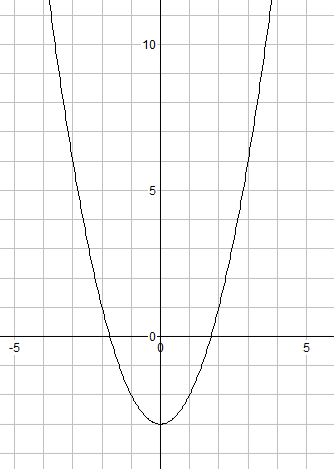
\includegraphics[ width=2.0496in, height=2.8669in,]{L4SZ2709}
}
\\ 
\\



\begin{tabular}[c]{rrlr}14.  &  & $3.61$  &  \\
	&  &  &  \\
	15.
	&  & x-intercepts $1.73$ and $ -1.73$  &  \\
	&  & y-intercept
	$ -3$  &  \\
	&  &  &  \\
	16.
	& (a)  & On the graph below  &  \\
	& (b)
	& $2$  &  \\
	& (c)
	& $y =2 x -1$  &  \\
	& (d)
	& $y =2 x +7$  & 
\end{tabular}

16. (e)
\setlength\fboxrule{0.01in}\setlength\fboxsep{0.2in}\fcolorbox[HTML]{000000}{FFFFFF}{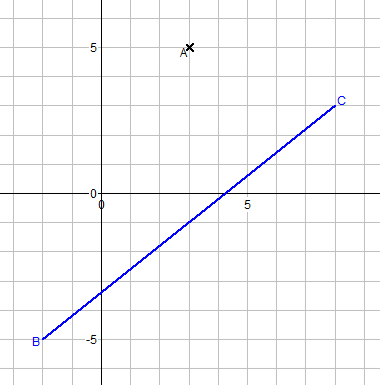
\includegraphics[ width=2.8297in, height=2.8669in,]{L4SZ270A}
}
\\ 
\\



\begin{tabular}[c]{rrrr}17.  & (a)
	& $4$  &  \\
	& (b)
	& $4$  &  \\
	& (c)
	& $27$  &  \\
	& (d)
	& $ -27$  & 
\end{tabular}

18.
\begin{tabular}[c]{|c|c|}\hline
	$x$  & $g (x) =x^{3} -x$  \\
	\hline
	$ -1.5$  & $ -1.875\;$  \\
	\hline
	$ -1$  & $0$  \\
	\hline
	$ -0.5$  & $0.375$  \\
	\hline
	$0$  & $0$  \\
	\hline
	$0.5$  & $ -0.375$  \\
	\hline
	$1$  & $0$  \\
	\hline
	$1.5$  & $1.875$  \\
	\hline
\end{tabular}\vspace{0.5cm} \\\relax
\setlength\fboxrule{0.01in}\setlength\fboxsep{0.2in}\fcolorbox[HTML]{000000}{FFFFFF}{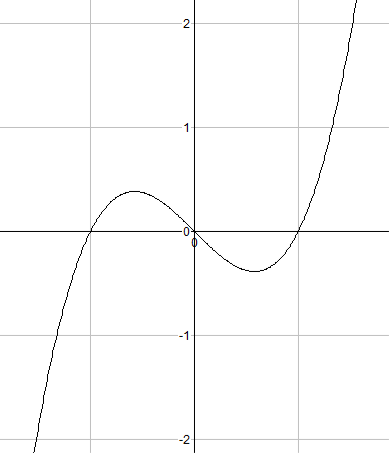
\includegraphics[ width=2.4656in, height=2.866in,]{L4SZ270B}
}


$
\begin{tabular}[c]{rrlr}19. 
& (a)
& $4$
& 
\\
& (b)
& $ -3$, $1$, $ -1$ (touches) 
& 
\\
& (c)
& $ -3$
& 
\end{tabular}\vspace{+0.500000cm}$ 

19.(d)    
\setlength\fboxrule{0.01in}\setlength\fboxsep{0.2in}\fcolorbox[HTML]{000000}{FFFFFF}{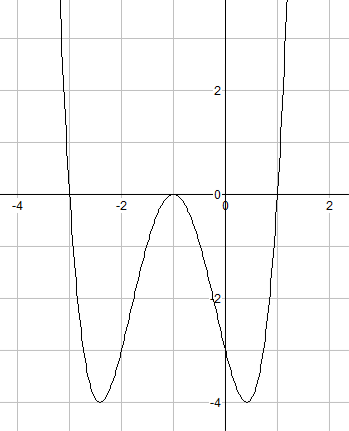
\includegraphics[ width=2.3263in, height=2.866in,]{L4SZ270C}
}


20. (a) $8 ,4 ,2 ,1 ,\frac{1}{2} ,\frac{1}{4} ,\frac{1}{8}\vspace{+0.500000cm}$ \\\relax    
\setlength\fboxrule{0.01in}\setlength\fboxsep{0.2in}\fcolorbox[HTML]{000000}{FFFFFF}{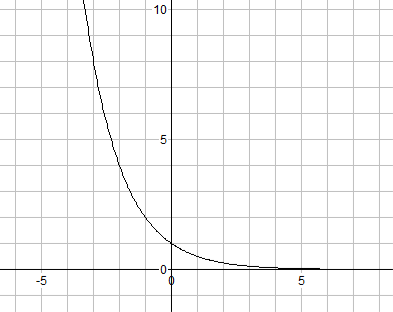
\includegraphics[ width=3.1782in, height=2.5278in,]{L4SZ270D}
}



\begin{tabular}[c]{rrrl}20.  & (b)
	& 1.  & $41.9$  \\
	&  & 2.
	& $0.5488$  \\
	&  &  &  \\
	21.
	& (a)  &  & $\log _{10} 0.01 = -2$  \\
	& (b)  & 1.
	& $625 =5^{4}$  \\
	&  & 2.
	& $k =a^{t}$  \\
	& (c)  & 1.
	& $1$  \\
	&  & 2.
	& $ -3$  \\
	&  & 3.
	& $3$  \\
	&  & 4.
	& $1.082$  \\
	&  & 5.
	& $3.1$  \\
	&  & 6.
	& $ -1$  \\
	&  &  &  \\
	22.
	& (a)  &  & $\log _{4} 35$  \\
	& (b)  &  & $\log _{5} 6$  \\
	& (c)  &  & $\log _{3} 16$  \\
	& (d)  &  & $\log _{4} 8$  \\
	&  &  &  \\

\end{tabular} 
\clearpage
\section{Factoring Exercises}
Some exercises look quite difficult on the surface but quickly look like a
familiar one once you get started. 

\subsubsection{Example}
Completely factor the following expression: $x^{4} +2 x^{3} -3 x^{2}$\\
Start by removing the common factor to all terms: $x^2$\\
\begin{eqnarray*} x^{4} +2 x^{3} -3 x^{2} &= x^{2} \left (x^{2} +2 x -3\right ) \\
	\text{then factor the remaining term as usual}\\
	 &= x^{2} \left (x -1\right ) \left (x +3\right )\end{eqnarray*}


Solve the following equations both algebraically and graphically.
*Note there are no answers for these exercises. Want to make some? Email them to Jeff!
\begin{enumerate}
	\item   
	\columnsep =30pt
	\begin {multicols}{2}
	$x -4 =5 x +12$ 
	
	\item $\frac{1}{2} x -3 =6 +2 x$ 
	
	\item $\frac{2}{x} +\frac{1}{2 x} =7$ 
	
	\item $\frac{4}{x +2} -\frac{6}{2 x} =\frac{5}{2 x +4}$ 
	
	\item $x^{2} -32 =0$ 
	
	\item $x^{3} +16 =0$ 
	
	\item $16 x^{4} =625$ 
	
	\item $2 x^{5} -243 =0$ 
	
	\item $\left (x -5\right )^{4} -80 =0$ 
	
	\item $6 \left (x +2\right )^{5} =64$ 
	\end {multicols}

\end{enumerate}


Find all real solutions of these equations correct to two decimal places (d.p.). 


\begin{enumerate}
	  
	\columnsep =30pt
	\begin {multicols}{2}\setcounter{enumi}{10}\item
	$x^{3} -2 x^{2} -x -1 =0$ 
	
	\item $x^{4} -8 x^{2} +2 =0$ 
	
	\item $x \left (x -1\right ) \left (x +2\right ) =\frac{1}{6} x$ 
	
	\item $x^{4} =16 -x^{3}$ 
	\end {multicols}

\end{enumerate}


Solve these inequalities correct to two d.p. 
\begin{enumerate}
	\setcounter{enumi}{14}\item   
	\columnsep =30pt
	\begin {multicols}{2}
	$x^{2} -3 x -10 \leq 0$ 
	
	\item $0.5 x^{2} +0.875 x \leq 0.25$ 
	
	\item  $x^{3} +11 x \leq 6 x^{2} +6$ 
	
	\item $16 x^{3} +24 x^{2} > -9 x -1$ 
	
	\item  $x^{\frac{1}{3}} <x$ 
	
	\item  $\left (x +1\right )^{2} <\left (x -1\right )^{2}$ 
	\end {multicols}

\end{enumerate}
